\newpage
\section*{Appendix C: Simulation study}\label{subsec:sim-study}

We present a simulation study to assess the ability of the proposed model to correctly estimate the parameters and the clustering of the areal units. Using the model introduced in Section \ref{subsec:Label-Assignment}, we simulate data for a grid of $10 \times 10$ areal units.

The adjacency structure is induced by contiguity on the grid (units are treated as neighbors if they share a boundary). The spatial effect $\phi_i$ is simulated fixing $\tau = 1$ and $\rho = 0.9$. Conditional on a fixed true partition, each unit $i$ is assigned a vector of covariates $x_i \in \mathbb{R}^{P}$, with $P=2$ in the implementation, generated independently from a Gaussian distribution. Given the true cluster membership $k \in \{1,\dots,K_0\}$, the response is then generated from a cluster-specific linear regression model:
\[
y_i = \phi_i + x_i^\top \beta_{k} + \varepsilon_i \, , 
\qquad \varepsilon_i \sim \mathcal{N}(0,1),
\]
where $\beta_k$ varies across clusters. In the experiments below we report results for two configurations of the true cluster structure (a simpler setting with $K_0=4$ clusters and a more complex setting with $K_0=7$ clusters), corresponding to the maps displayed in Figures~\ref{fig:true-vs-pred-k4} and \ref{fig:true-vs-pred-k7}.

Posterior sampling is carried out via Hamiltonian Monte Carlo using four chains, 5,000 warm-up iterations and 5,000 retained iterations per chain. Cluster labels are produced at each posterior draw through the label-assignment step described in Section~\ref{subsec:Label-Assignment}.\\

Figure~\ref{fig:psm} shows a clear block-diagonal structure in the PSM, indicating that the posterior assigns high co-clustering probability to units within the same true region, while keeping between-region probabilities close to zero. This qualitative pattern is reflected in the spatial maps: in the simpler $K_0=4$ setting, the estimated partition aligns perfectly with the ground truth (Figure~\ref{fig:true-vs-pred-k4}). Moreover the density plots (Figure \ref{fig:betaposterior-true}) show that the true $\beta$ coefficients are accurately recovered.

In the more heterogeneous configuration, the selected partition yields $K=7$ clusters and recovers the overall structure (Figure~\ref{fig:true-vs-pred-k7}). Discrepancies are limited to a small subset of units and are concentrated at the borders between neighboring clusters; in addition, the distinction between two true clusters is essentially lost, as these regions are largely merged into a single estimated cluster in the predicted map.


\begin{figure}[H]
  \centering
  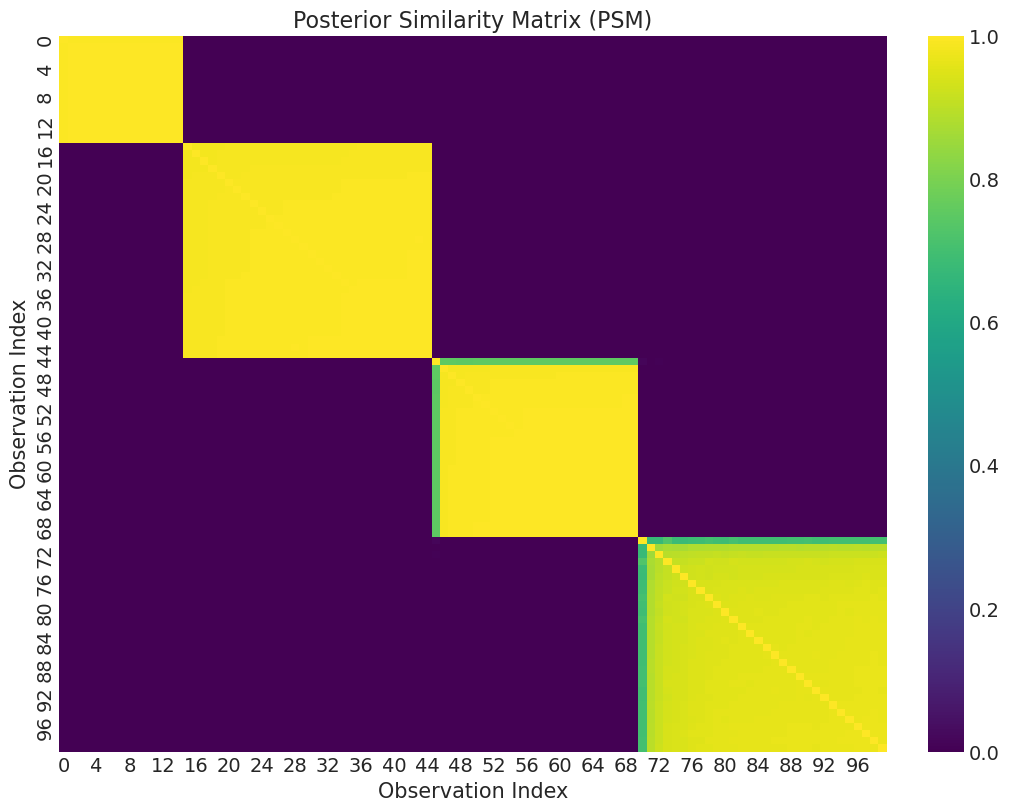
\includegraphics[width=0.65\textwidth]{chapters/images/psm-k4.png}
  \caption{Posterior similarity matrix (PSM) for the simulated data when $K_0 = 4$.}
  \label{fig:psm}
\end{figure}

\begin{figure}[H]
  \centering
  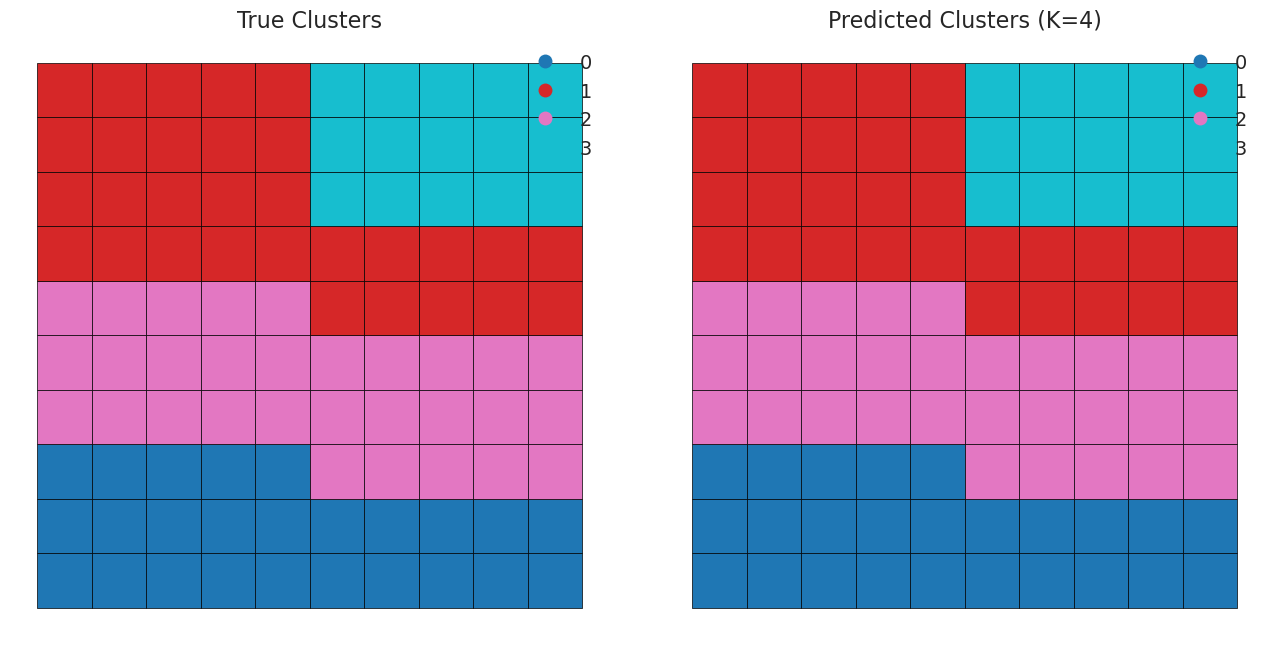
\includegraphics[width=0.8\textwidth]{chapters/images/comparison-k4.png}
  \caption{True clusters (left) and estimated clusters (right) for the $K_0=4$ configuration.}
  \label{fig:true-vs-pred-k4}
\end{figure}

\begin{figure}[H]
  \centering
  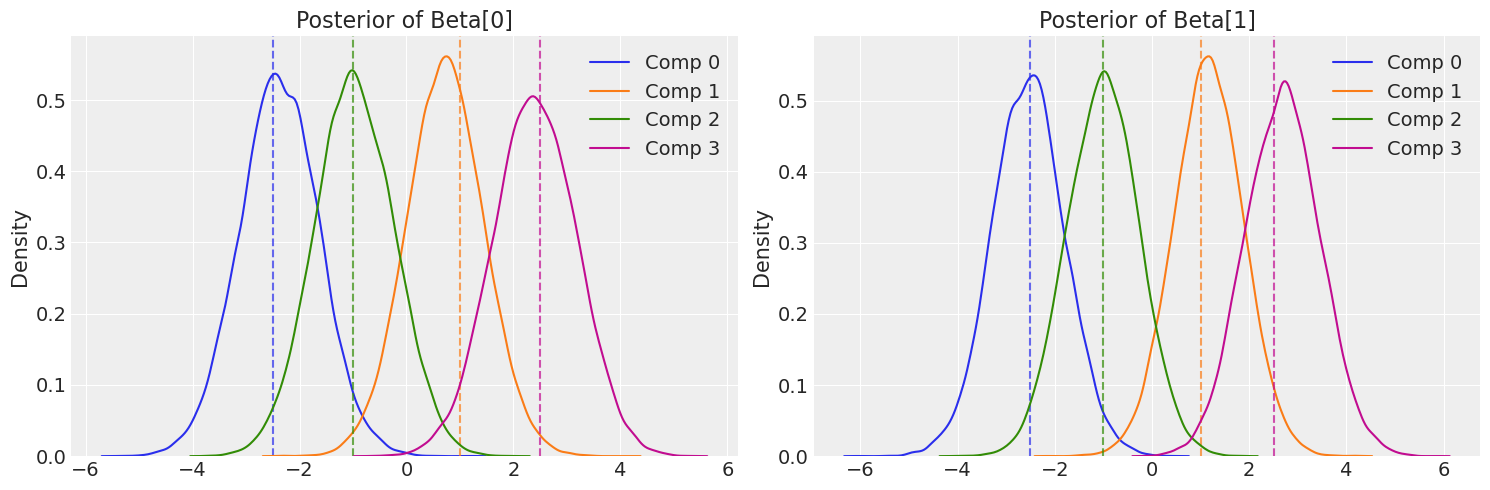
\includegraphics[width=1\textwidth]{chapters/images/betaposterior-truevalue.png}
  \caption{Posterior density of the cluster-specific regression coefficients $\beta$ and their true value for the $K_0 = 4$ configuration.}
  \label{fig:betaposterior-true}
\end{figure}

\begin{figure}[htbp]
\centering
  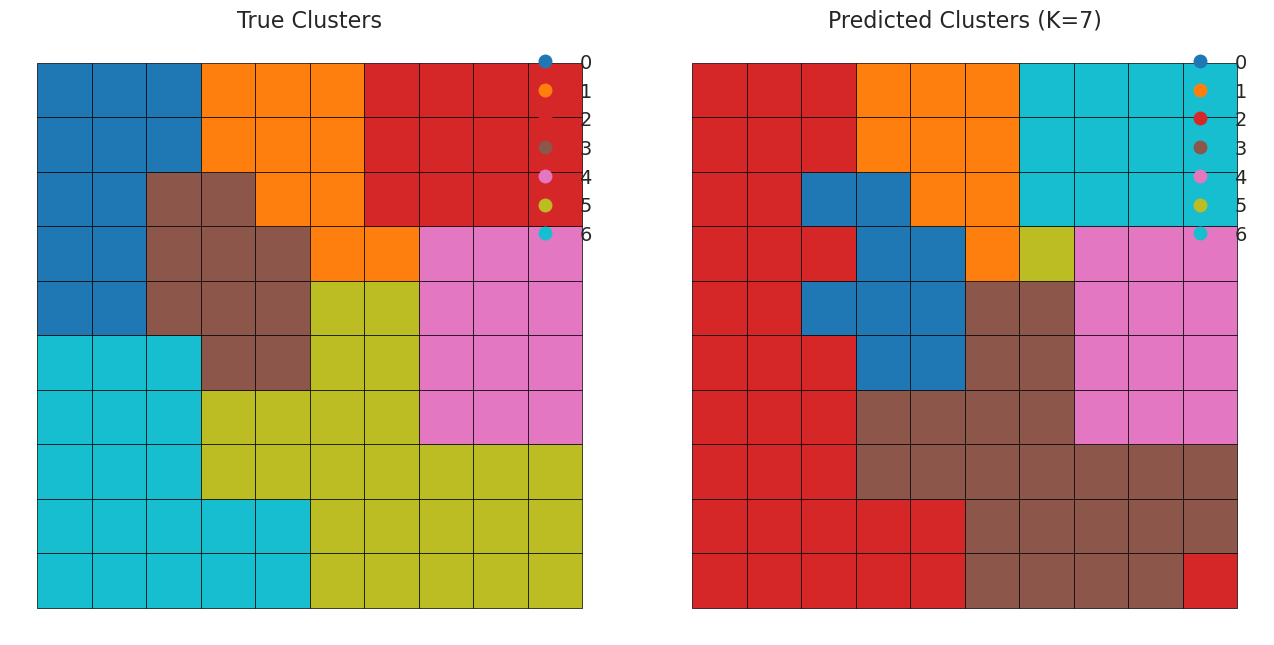
\includegraphics[width=0.8\textwidth]{chapters/images/comparison-k7.png}
  \caption{True clusters (left) and estimated clusters (right) for the for the configuration with $K_0 = 7$.}
  \label{fig:true-vs-pred-k7}
\end{figure}

